\documentclass[]{article}
\usepackage{graphicx}

%opening
\title{Supplementary material: Dynamic cancer drivers: A causal approach for cancer driver discovery based on bio-pathological trajectories}
\author{Andres M. Cifuentes-Bernal$^{{ }1}$\and, Vu VH Pham$^{1}$,\and Xiaomei Li$^{1}$,\and Lin Liu$^{1}$,\and Jiuyong Li$^{ 1}$ \and and Thuc Duy Le$^{1*}$}
\date{$^1$ UniSA STEM, University of South Australia, Adelaide, 5095 Mawson Lakes SA, Australia.\\ $^{1*}$ \small{Correspondence author: thuc.le@unisa.edu.au}}



\begin{document}

\maketitle

\section{GO biological processes analysis}

We performed a GO biological processes enrichment analysis to the single cell RNA sequencing data from NCBI GEO database, accession GSE75688  \cite{Chung2017} to verify how significantly related are our discoveries to processes in cancer. Our analyses show a significant number of discovered
drivers are strongly related relevant biological processes in cancer disease. Top ten enriched terms (for each trajectory) from Go Biological
Processes are shown in Fig. \ref{fig:vimher2gobiologicalprocess2021} . For both dynamic drivers inferred sets (i.e from VIMtime(SC), and HER2time(SC)), top 10 enriched terms (ranked by p-value) are relevant to cancer (e.g.
regulation of transcription and regulation of apoptotic process).

\begin{figure}[h]
	\centering
	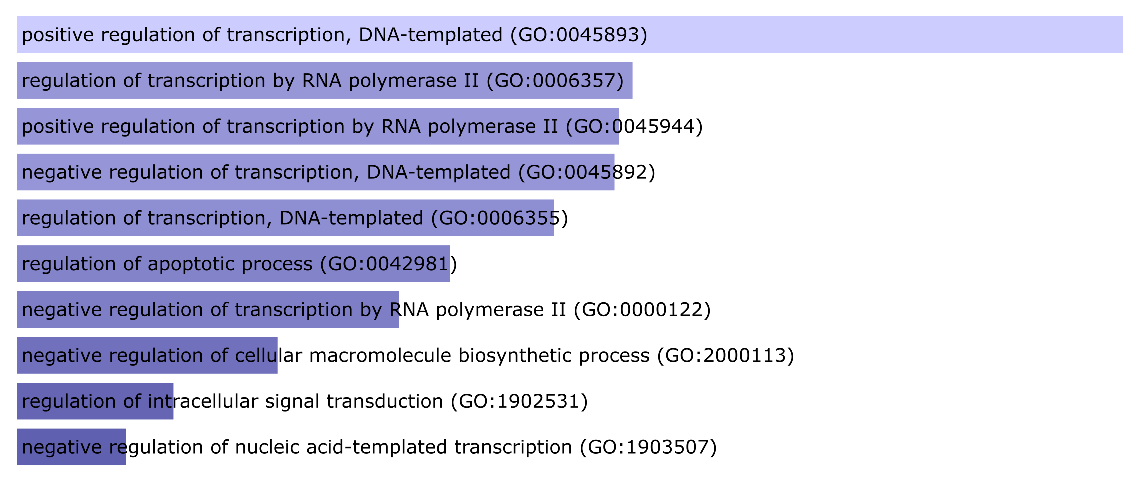
\includegraphics[width=0.8\linewidth]{./GO_Biological_Process_2021_bar_SC_VIM06.eps}
	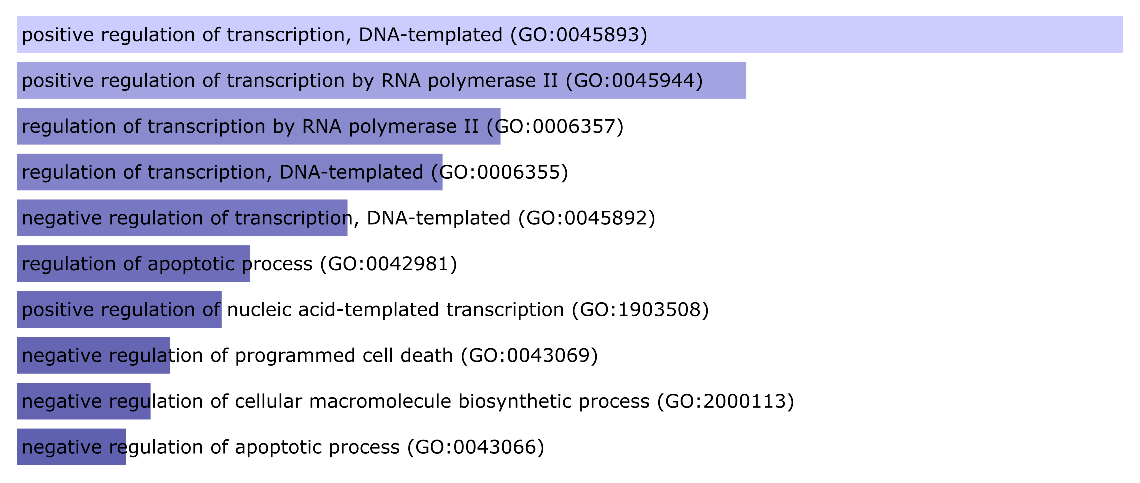
\includegraphics[width=0.8\linewidth]{./GO_Biological_Process_2021_bar_SC_HER206.eps}
	\caption{Top 10 Go biological terms 2021 (ranked by p-value) from our enrichment analysis for the gene set obtained from "VIMtime(SC)" (upper) and "HER2time(SC)" (lower). In both cases, enriched terms correspond to regulation of biological processes relevant to cancer progression. Bar length represents the significance of the term. Brightness is used as auxiliary visual for significance, the lower the p-value, the brighter the colour. Analysis performed by using Enrichr \cite{Kuleshov2016}}
	\label{fig:vimher2gobiologicalprocess2021}
\end{figure}

\newpage
\section{Gene-disease association analysis (DisGeNet)}

 \begin{figure}[h]
	\centering
	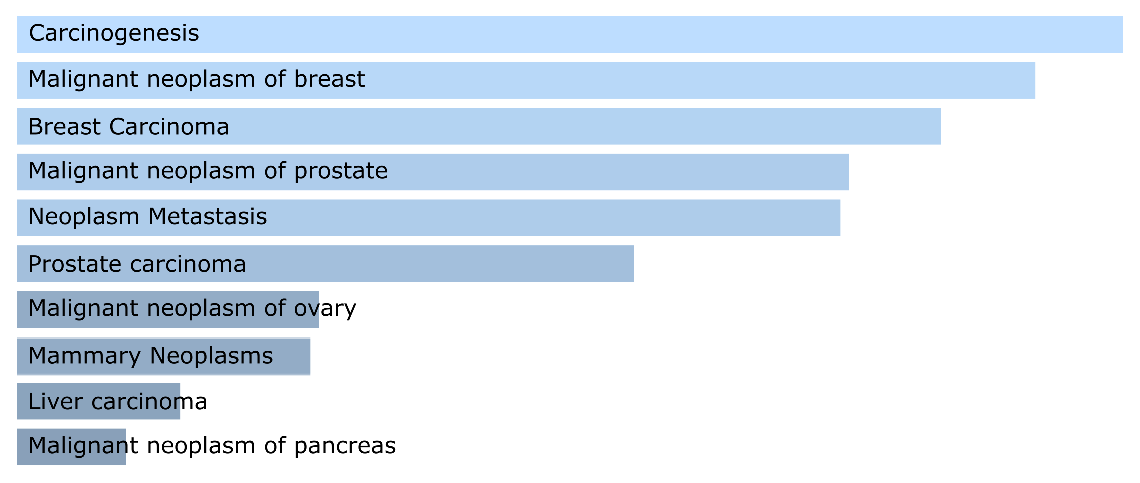
\includegraphics[width=0.8\linewidth]{./DisGeNET_bar_SC_VIM06.eps}
	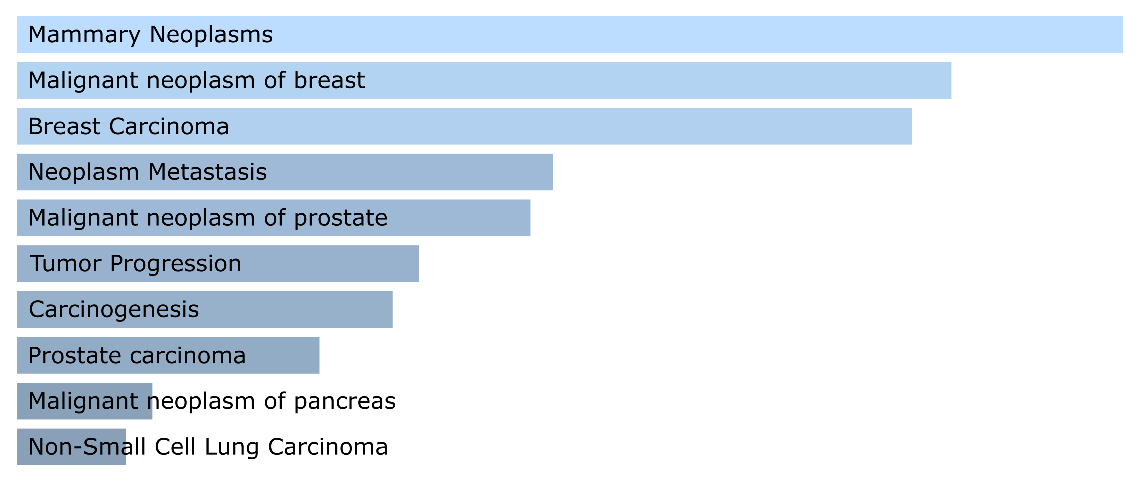
\includegraphics[width=0.8\linewidth]{./DisGeNET_bar_SC_HER206.eps}
	\caption{Top 10 GDAs terms (ranked by p-value) from our enrichment analysis for the gene set obtained from "VIMtime(SC)" (upper) and "HER2time(SC)" (lower) retrieved from DisGeNET. Bar length represents the significance of the term. Brightness is used as auxiliary visual for significance, the lower the p-value, the brighter the colour. Analysis performed by using Enrichr \cite{Kuleshov2016}}
	\label{fig:disgenetbargraphsc}
\end{figure}

We performed an enrichment analysis to identify gene-disease associations (GDAs) in the inferred drivers from the GSE75688 single cell dataset  \cite{Chung2017}. We use DisGeNET \cite{Pinero2016} as gene-disease associations database for this analysis. Our analyses show a significant number of discovered drivers are strongly related to cancer disease. The top ten enriched GDAs terms (ranked by p-value) for each of the analysed pseudotimes (i.e VIMtime(SC), and HER2time(SC)) are shown in Fig. \ref{fig:disgenetbargraphsc}. In both cases, all of top ten terms are related to cancer disease and cancer progression.




\newpage


\bibliography{references}
\bibliographystyle{apalike}
\end{document}
